\documentclass[12pt]{article}
\usepackage{amsmath}
\usepackage{amssymb}
\usepackage{geometry}
\usepackage{amsmath, amsfonts, bm, graphicx}
\usepackage{tabularx}
\usepackage{booktabs} 
\usepackage{float}
\usepackage{enumitem}
\geometry{margin=1in}

\title{}
\date{}
\author{}

\begin{document}
\subsection*{\boxed{\text{HW 5 - Zeshui Song}}}

\section*{7.4}
\vspace{-2em}
\begin{center}
    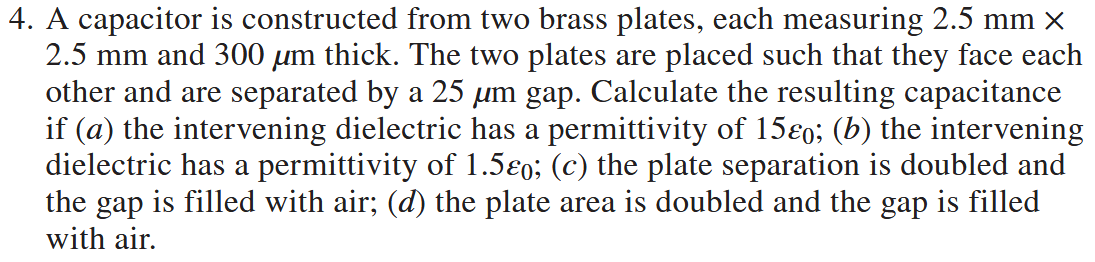
\includegraphics[width=0.8\textwidth]{7-4.png}
\end{center}
\vspace{-1em}
The capacitance of a parallel-plate capacitor is given by the formula:
\[C =  \frac{\varepsilon_0 \varepsilon_rA}{d}\]
Where $\varepsilon_0=8.854 \times 10^{-12} \, \text{F/m}$ is the permittivity of free space, $\varepsilon_r$ is the relative permittivity of the dielectric material, $A$ is the area of the plates, and $d$ is the distance between the plates.\\\\
\textbf{(a) $\varepsilon_r=15$, $A=6.25 \, \text{mm}^2$, $d=25 \, \mu\text{m}$}
\[C =  \frac{15\varepsilon_0A}{d} = \frac{15[8.854 \times 10^{-12}\, \text{F/m}]\left[6.25\,\text{mm}^2 \cdot \frac{(10^{-3} m )^2}{1\,\text{mm}^2}\right]}{[25 \times 10^{-6}\, \text{m}]}=\boxed{3.3202\times10^{-11}\,\text{F}}\]
\textbf{(b) $\varepsilon_r=1.5$, $A=6.25 \, \text{mm}^2$, $d=25 \, \mu\text{m}$}
\[C =  \frac{1.5\varepsilon_0A}{d} = \frac{1.5[8.854 \times 10^{-12}\, \text{F/m}]\left[6.25\,\text{mm}^2 \cdot \frac{(10^{-3} m )^2}{1\,\text{mm}^2}\right]}{[25 \times 10^{-6}\, \text{m}]}=\boxed{3.3202\times10^{-12}\,\text{F}}\]
\textbf{(c) $\varepsilon_r=1$ (air), $A=6.25 \, \text{mm}^2$, $d=50 \, \mu\text{m}$}
\[C =  \frac{\varepsilon_0A}{d} = \frac{[8.854 \times 10^{-12}\, \text{F/m}]\left[6.25\,\text{mm}^2 \cdot \frac{(10^{-3} m )^2}{1\,\text{mm}^2}\right]}{[50 \times 10^{-6}\, \text{m}]}=\boxed{1.1067\times10^{-12}\,\text{F}}\]
\textbf{(d) $\varepsilon_r=1$ (air), $A=12.5 \, \text{mm}^2$, $d=25 \, \mu\text{m}$}
\[C =  \frac{\varepsilon_0A}{d} = \frac{[8.854 \times 10^{-12}\, \text{F/m}]\left[12.5\,\text{mm}^2 \cdot \frac{(10^{-3} m )^2}{1\,\text{mm}^2}\right]}{[25 \times 10^{-6}\, \text{m}]}=\boxed{4.427\times10^{-12}\,\text{F}}\]

\section*{7.9}
\vspace{-2em}
\begin{center}
    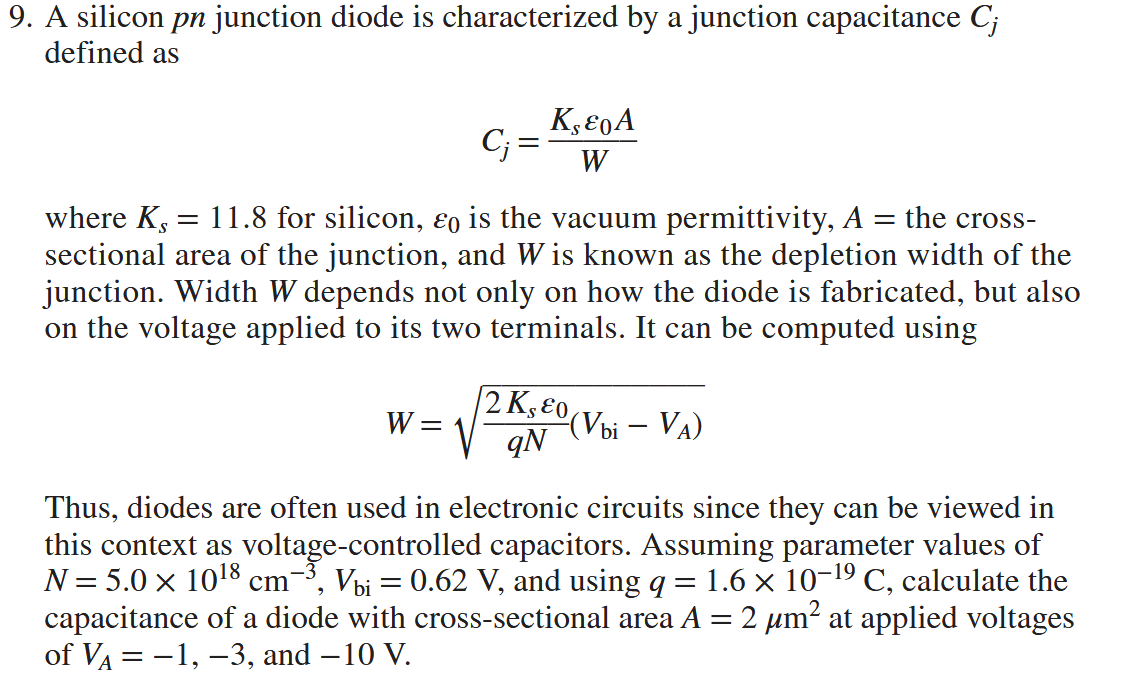
\includegraphics[width=0.8\textwidth]{7-9.png}
\end{center}
\vspace{-1em}
Rewriting the formula for capacitance:
\[C_j = K_s\varepsilon_0 A \sqrt{\frac{qN}{2K_s \varepsilon_0 (V_{bi}-V_A)}} = A\sqrt{\frac{K_s^2\varepsilon_0^2qN}{2K_s \varepsilon_0 (V_{bi}-V_A)}} = A\sqrt{\frac{K_s\varepsilon_0qN}{2 (V_{bi}-V_A)}}\]
\[C_j = \left[2\,\mu\text{m}^2\cdot\frac{(10^{-6}\,\text{m})^2}{1\mu\text{m}^2}\right]\sqrt{\frac{[11.8][8.854 \times 10^{-12}\, \text{F/m}][1.6\times10^{-19}\,\text{C}]\left[5\times10^{18}\,\text{cm}^{-3}\cdot\frac{(10^{-2}\,\text{m})^{-3}}{1\,\text{cm}^{-3}}\right]}{2 ([0.62\,\text{V}]-V_A)}}\]
\[C_j  = (2\times10^{-12})\sqrt{\frac{8.3581\times10^{-5}}{2 ([0.62\,\text{V}]-V_A)}} \,[\text{F}]\]
\underline{Note:} 1 F = 1 C/V. \\\\
\textbf{(a) $V_A = -1$ V}
\[C_j  = (2\times10^{-12})\sqrt{\frac{8.3581\times10^{-5}}{2 ([0.62- (-1)\,\text{V}])}}= \boxed{1.0158\times10^{-14} \,\text{F}}\]
\textbf{(b) $V_A = -3$ V}
\[C_j  = (2\times10^{-12})\sqrt{\frac{8.3581\times10^{-5}}{2 ([0.62- (-3)\,\text{V}])}}= \boxed{6.7954\times10^{-15} \,\text{F}}\]
\textbf{(c) $V_A = -10$ V}
\[C_j  = (2\times10^{-12})\sqrt{\frac{8.3581\times10^{-5}}{2 ([0.62- (-10)\,\text{V}])}}= \boxed{3.9674\times10^{-15} \,\text{F}}\]

\section*{7.11}
\vspace{-2em}
\begin{center}
    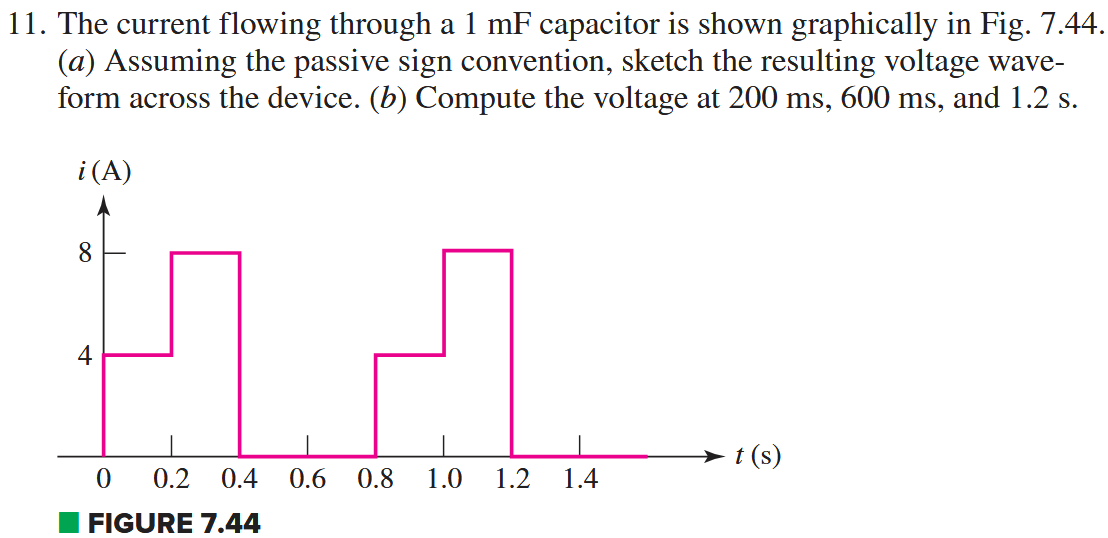
\includegraphics[width=0.8\textwidth]{7-11.png}
\end{center}
\vspace{-1em}
The voltage over a capacitor is given by the formula:
\[V = \frac{Q}{C} = \frac{\int i(t)\,dt}{C} = \frac{i}{C}t\]
\underline{Note:} Passive sign convention means that the capacitor is absorbing current (charging), so in the context of KVL, there will be a voltage drop in the direction of the current.\\\\
\textbf{(a)} Since the current is constant at varying amplitudes, the voltage across the capacitor will increase with different slopes (higher current will lead to a steeper slope).
\begin{center}
    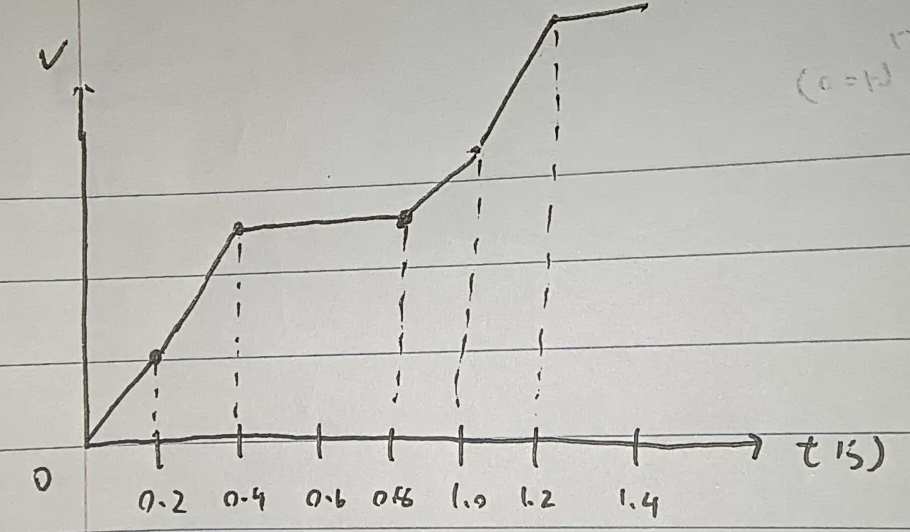
\includegraphics[width=0.4\textwidth]{7-11_1.png}
\end{center}
\textbf{(b)} We can sum up the charge accumulated in the capacitor at each time interval to find the voltage across the capacitor at each time.
\[V_{t=0\to0.2} = \frac{[4\,\text{A}][0.2\,\text{s}]}{[10^{-3}\,\text{F}]} = \boxed{800\,\text{V}\quad\text{(at 200 ms)}}\]
\[V_{t=0\to0.4} = V_{t=0\to0.2}+ \frac{[8\,\text{A}][0.2\,\text{s}]}{[10^{-3}\,\text{F}]} = \boxed{2400\,\text{V}\quad\text{(at 600 ms)}}\]
\[V_{t=0\to1.2} = V_{t=0\to0.4}+ \frac{[4\,\text{A}][0.2\,\text{s}]}{[10^{-3}\,\text{F}]}+\frac{[8\,\text{A}][0.2\,\text{s}]}{[10^{-3}\,\text{F}]} = \boxed{4800 \,\text{V}\quad\text{(at 1.2 s)}}\]

\newpage

\section*{7.13}
\vspace{-2em}
\begin{center}
    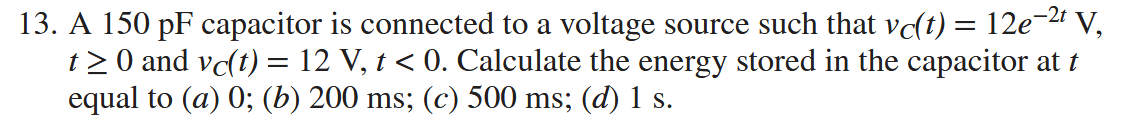
\includegraphics[width=0.8\textwidth]{7-13.png}
\end{center}
\vspace{-1em}
The energy stored in a capacitor is given by the formula:
\[w = \frac{1}{2}CV^2(t) = \frac{q^2(t)}{2C}\]
\textbf{(a)} at $t=0$ s
\[w = \frac{1}{2}[150\times10^{-12}\,\text{F}](12e^{-2})^2= \boxed{10.8\times10^{-9}\,\text{J}}\]
\textbf{(b)} at $t=0.2$ s
\[w = \frac{1}{2}[150\times10^{-12}\,\text{F}](12e^{-0.4})^2= \boxed{4.852  \times10^{-9}\,\text{J}}\]
\textbf{(c)} at $t=0.5$ s
\[w = \frac{1}{2}[150\times10^{-12}\,\text{F}](12e^{-1})^2= \boxed{1.4616\times10^{-9}\,\text{J}}\]
\textbf{(d)} at $t=1$ s
\[w = \frac{1}{2}[150\times10^{-12}\,\text{F}](12e^{-2})^2= \boxed{0.1978  \times10^{-9}\,\text{J}}\]

\section*{7.15}
\vspace{-2em}
\begin{center}
    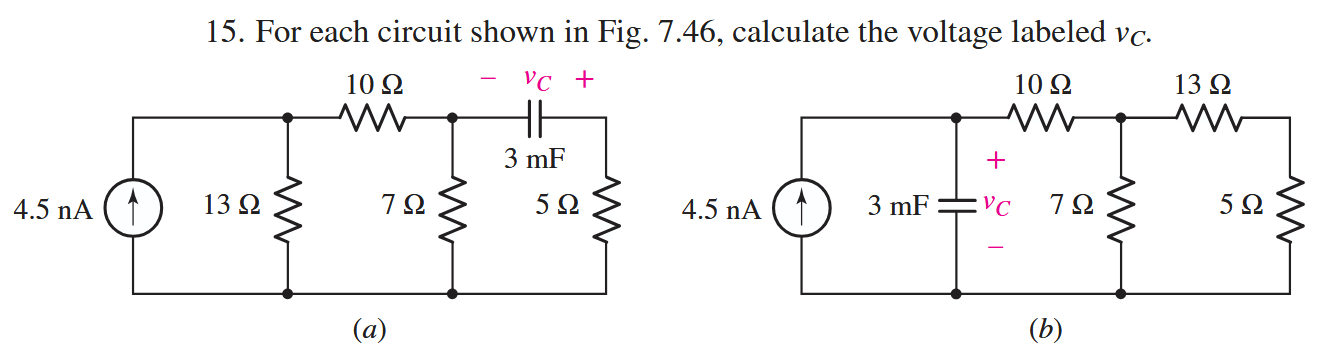
\includegraphics[width=0.8\textwidth]{7-15.png}
\end{center}
\vspace{-1em}
Assuming that the circuit is in steady state, the capacitor will act like an open circuit, with no current flowing through it.\\\\
\textbf{(a)} Start with a source transformation of the current source to a voltage source:
\[V_s = i_s R_s = [4.5\times10^{-9}\,\text{A}][13\,\Omega]=5.85\times10^{-8}\,\text{V}\]
\[R_s = R_p = 13\,\Omega\]
\begin{center}
    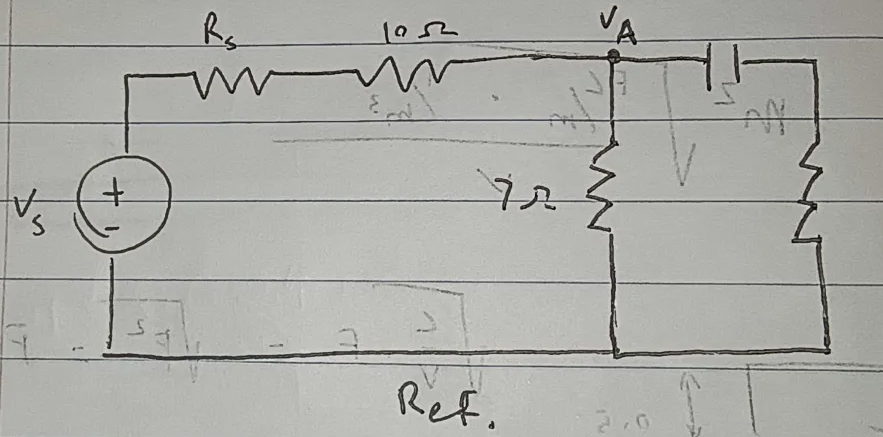
\includegraphics[width=0.5\textwidth]{7-15_1.png}
\end{center}
Thus, the current through the capacitor will be equal to the voltage over the 7 $\Omega$ resistor. We can find it using voltage division:\\\\
Combine the $R_s$ and $10\,\Omega$ resistor in series:
\[R = 13+10\,\Omega = 23\,\Omega\]
\[V_{7\Omega} = [5.85\times10^{-8}\,\text{V}] \cdot \frac{7\,\Omega}{7\,\Omega + 23\,\Omega} = 1.365\times10^{-8}\,\text{V}\]
Since the diagram shows the negative terminal of $V_c$ is equal to the positive terminal of $V_{7\Omega}$, the voltage across the capacitor has to be negative. This also makes sense since it is resisting the current flow from the voltage source, so it will be charged in the opposite direction of the voltage source.
\[\implies \boxed{V_c = -1.365\times10^{-8}\,\text{V}}\]
\textbf{(b)} The voltage over the capacitor is equal to the voltage over the current source. Thus, we start by finding the equivalent resistance of the circuit:\\\\
Combine 13 $\Omega$ and 5 $\Omega$ in series:
\[R_1 = 13 + 5\,\Omega = 18\,\Omega\]
Combine $R_1=18\,\Omega$ and 7 $\Omega$ in parallel:
\[R_2 = \frac{18\cdot7}{18+7}\,\Omega = 5.04\,\Omega\]
Combine $R_2=5.04\,\Omega$ and 10 $\Omega$ in series:
\[R_{eq} = 5.04 + 10\,\Omega = 15.04\,\Omega\]
Thus, the voltage across the current source is:
\[V_s = i_s R_{eq} = [4.5\times10^{-9}\,\text{A}][15.04\,\Omega] = 6.768\times10^{-8}\,\text{V}\]
Based on the polarity of the capacitor:
\[\implies \boxed{V_c = 6.768\times10^{-8}\,\text{V}}\]

\section*{7.17}
\vspace{-2em}
\begin{center}
    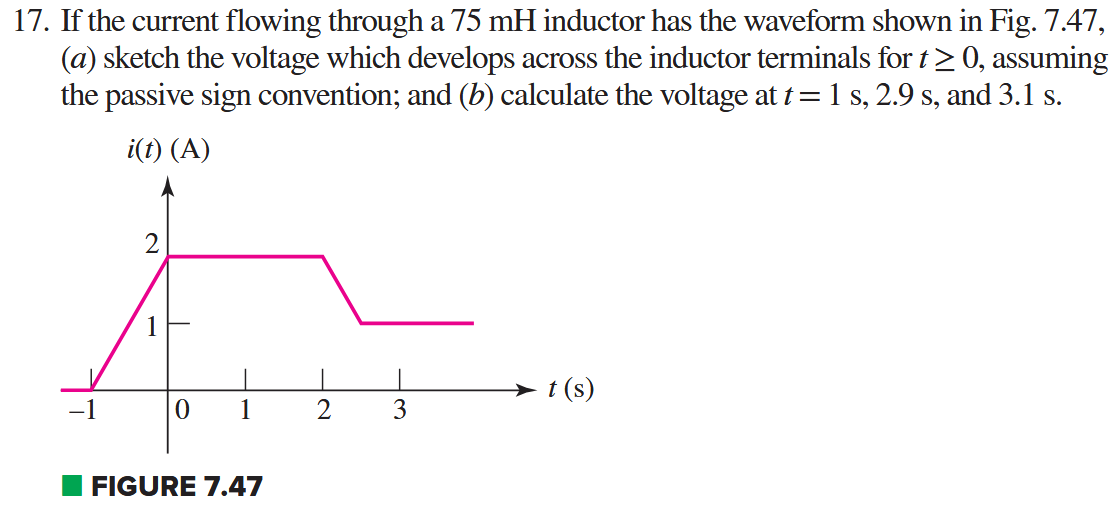
\includegraphics[width=0.8\textwidth]{7-17.png}
\end{center}
\vspace{-1em}
The voltage over an inductor is given by the formula:
\[V = L\frac{di}{dt}\]
Since the slopes of the current time plot are constant, the voltage across the inductor will be a step function, with the voltage being positive when the current is increasing and negative when the current is decreasing.\\\\
\textbf{(a)} 
\begin{center}
    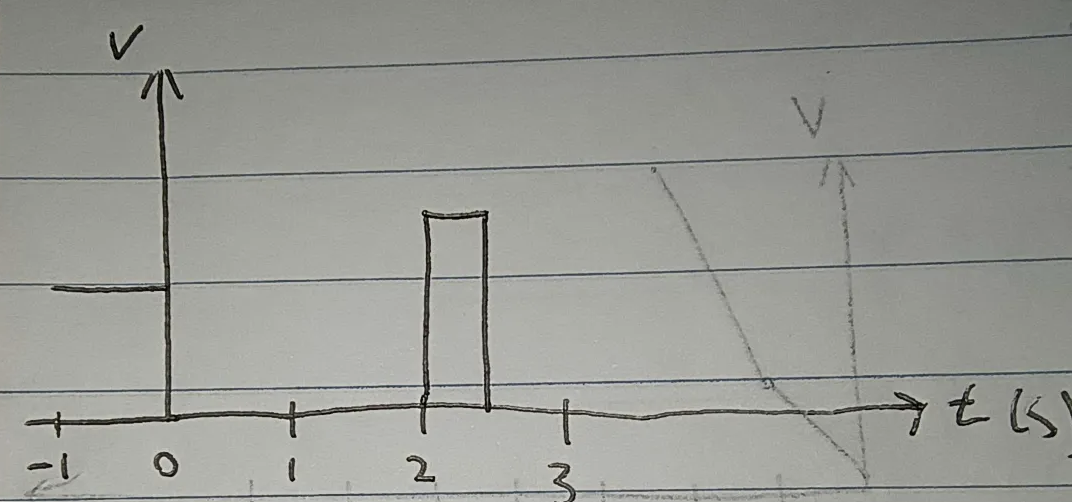
\includegraphics[width=0.5\textwidth]{7-17_1.png}
\end{center}
\textbf{(b)}
\[V(t=1) = L \left.\frac{di}{dt}\right|_{t=1}=[75\times10^{-3}\,\text{H}](0)=\boxed{0\,\text{V}}\]
\[V(t=2.9) = L \left.\frac{di}{dt}\right|_{t=2.9}=[75\times10^{-3}\,\text{H}](0)=\boxed{0\,\text{V}}\]
\[V(t=3.1) = L \left.\frac{di}{dt}\right|_{t=3.1}=[75\times10^{-3}\,\text{H}](0)=\boxed{0\,\text{V}}\]

\section*{7.21}
\begin{center}
    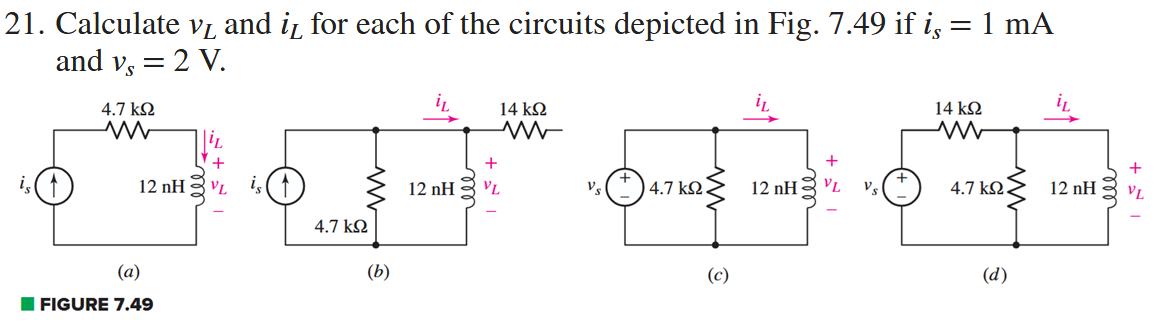
\includegraphics[width=1\textwidth]{7-21.png}
\end{center}
\vspace{-1em}
The voltage over an inductor is given by the formula:
\[V = L\frac{di}{dt}\]
Note that because the current in each circuit is constant, $\frac{di}{dt}=0$, so the voltage across the inductor will be zero in all cases. This means that the inductor will act like a short circuit, and the voltage across it will be zero.
\newpage\noindent
\textbf{(a)} 
\[\boxed{V_L = 0\,\text{V}}\]
\[\boxed{i_L = i_s = 1\,\text{mA}}\]
\textbf{(b)}
\[\boxed{V_L = 0\,\text{V}}\]
The inductor acts like a short, so all the current will flow through it instead (path of least resistance):
\[\boxed{i_L = i_s = 1\,\text{mA}}\]
\textbf{(c)}
\[\boxed{V_L = 0\,\text{V}}\]
Beacuse we basically shorted the voltage source, the current will be infinite across the inductor:
\[\boxed{i_L = \infty\,\text{mA}}\]
\textbf{(d)}
\[\boxed{V_L = 0\,\text{V}}\]
Using Ohm's law, we can find the current in the circuit. The 14 k$\Omega$ resistor has a voltage drop equal to the voltage source, because no current flows through the 4.7 k$\Omega$ resistor since the inductor is a short circuit:
\[v_s = i_L [14\,\text{k}\Omega] \implies i_L = \frac{v_s}{14\,\text{k}\Omega} = \frac{2\,\text{V}}{14\times10^3\,\Omega}=1.428\times10^{-4}\,\text{A}\]
\[\boxed{i_L = 0.1428\,\text{mA}}\]

\section*{7.26}
\vspace{-2em}
\begin{center}
    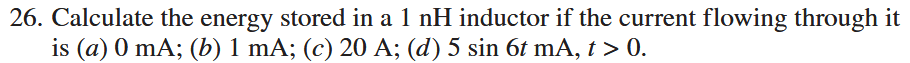
\includegraphics[width=0.8\textwidth]{7-26.png}
\end{center}
\vspace{-1em}
The energy stored in an inductor is given by the formula:
\[w=\frac{1}{2}Li^2(t)\]
\textbf{(a)} $i=0$ mA
\[\boxed{w=\frac{1}{2}Li^2(t)=\frac{1}{2}[10^{-9}\,\text{H}][0\,\text{A}]^2=0\,\text{J}}\]
\textbf{(b)} $i=1$ mA
\[\boxed{w=\frac{1}{2}Li^2(t)=\frac{1}{2}[10^{-9}\,\text{H}][10^{-3}\,\text{A}]^2=5\times10^{-16}\,\text{J}}\]
\textbf{(c)} $i=20$ A
\[\boxed{w=\frac{1}{2}Li^2(t)=\frac{1}{2}[10^{-9}\,\text{H}][20\,\text{A}]^2=0.2\times10^{-6}\,\text{J}}\]
\textbf{(d)} $i=5\sin(6t)$ mA
\[\boxed{w=\frac{1}{2}Li^2(t)=\frac{1}{2}[10^{-9}\,\text{H}][5\times10^{-3}\sin(6t)\,\text{A}]^2=1.25\times10^{-14}\sin^2(6t)\,\text{J}}\]

\section*{7.28}
\vspace{-2em}
\begin{center}
    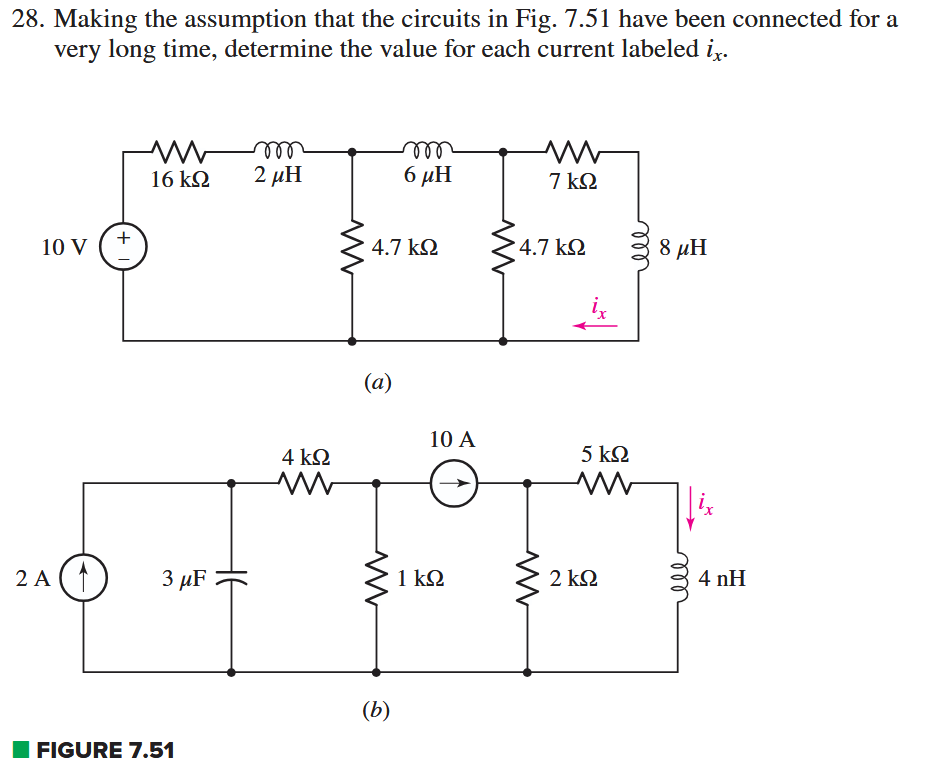
\includegraphics[width=0.8\textwidth]{7-28.png}
\end{center}
\vspace{-1em}
At steady state, the inductor will act like a short circuit with no resistance, so the voltage across it will be zero.\\\\
\textbf{(a)} The current $i_x$ can be found using Ohm's law if I can find the voltage over the 7 k$\Omega$ resistor. Since the inductor is like a short circuit (wire), the 7 k$\Omega$ and the two 4.7 k$\Omega$ resistors are in parallel so:
\[\frac{1}{R_1} = \frac{1}{7\,\text{k}\Omega} + \frac{1}{4.7\,\text{k}\Omega} + \frac{1}{4.7\,\text{k}\Omega} \implies R_1 = 1.759\,\text{k}\Omega\]
Now we just have resistor $R_1$ in series with the 16 k$\Omega$ resistor, so we can find the voltage over $R_1$ using voltage division:
\[V_{R_1} = v_s \cdot \frac{R_1}{R_1 + 16\,\text{k}\Omega} = [10\,\text{V}] \cdot \frac{[1.759\,\text{k}\Omega]}{[1.759 + 16\,\text{k}\Omega]} = 0.99066\,\text{V}\]
This voltage is the same as the voltage across the 7 k$\Omega$ resistor, since it is in parallel, so we can find the current $i_x$ using Ohm's law:
\[i_x = \frac{V_{R_1}}{7\,\text{k}\Omega} = \frac{[0.99066\,\text{V}]}{[7\times10^3\,\Omega]} = \boxed{1.415\times10^{-4}\,\text{A}}\]
\newpage\noindent
\textbf{(b)} At steady state, the capacitor becomes an open circuit as well. So we can redraw the circuit:
\begin{center}
    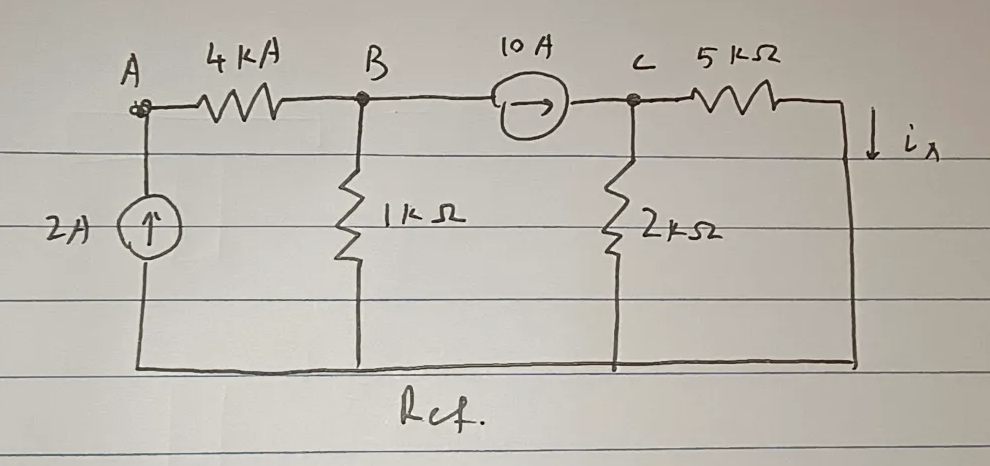
\includegraphics[width=0.6\textwidth]{7-28_1.png}
\end{center}
Using nodal analysis to find the voltage over the 5 k$\Omega$ resistor, we can find the current $i_y$ using Ohm's law.\\\\
KCL at node A:
\[[2\,\text{A}] = \frac{V_A-V_B}{[4\times10^3\,\Omega]}\]
KCL at node B:
\[\frac{V_A-V_B}{[4\times10^3\,\Omega]} = [10\,\text{A}] + \frac{V_B}{[10^3\,\Omega]}\]
KCL at node C:
\[[10\,\text{A}] = \frac{V_C}{[2\times10^3\,\Omega]} + \frac{V_C}{[5\times10^3\,\Omega]}\]
\[\implies V_C = 14485.714\,\text{V}\]
Using Ohm's law, we can find the current $i_x$:
\[i_y = \frac{V_C}{[5\times10^3\,\Omega]} = \frac{[14485.714\,\text{V}]}{[5\times10^3\,\Omega]} = \boxed{2.857\,\text{A}}\]

\section*{7.29}
\vspace{-2em}
\begin{center}
    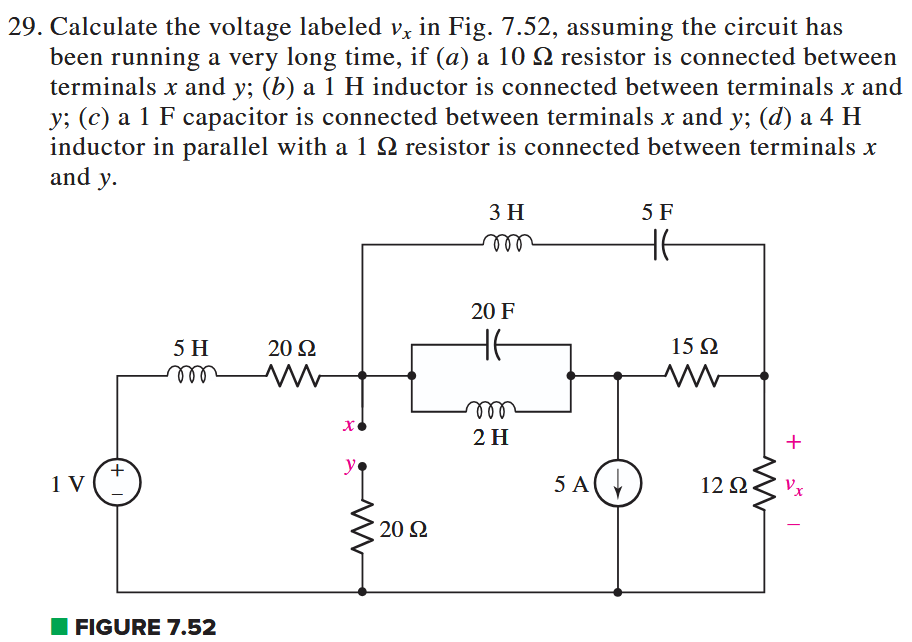
\includegraphics[width=0.8\textwidth]{7-29.png}
\end{center}
\vspace{-1em}
Redrawing the circuit at steady state:
\begin{center}
    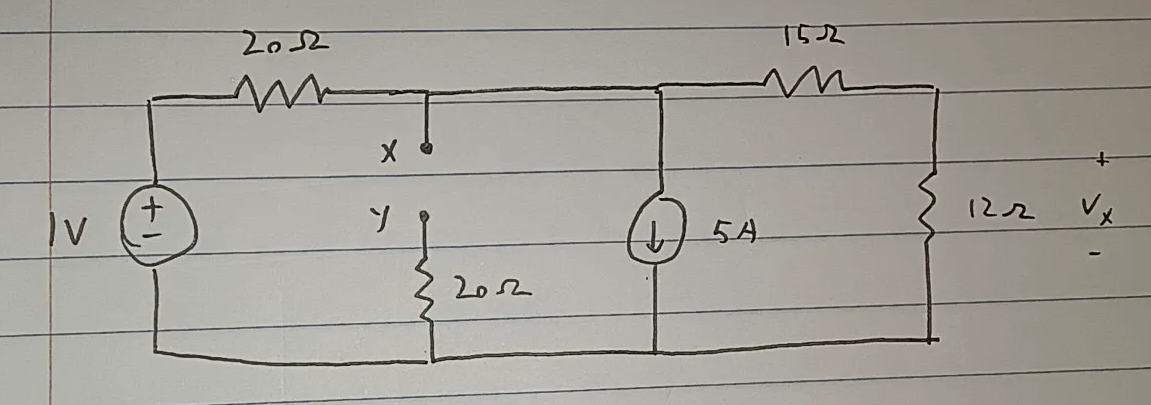
\includegraphics[width=0.6\textwidth]{7-29_1.png}
\end{center}
\textbf{(a)} Using nodal analysis, we can find $V_C=V_B$ and then use voltage division to find the voltage across the 12 $\Omega$ resistor $V_x$.
\begin{center}
    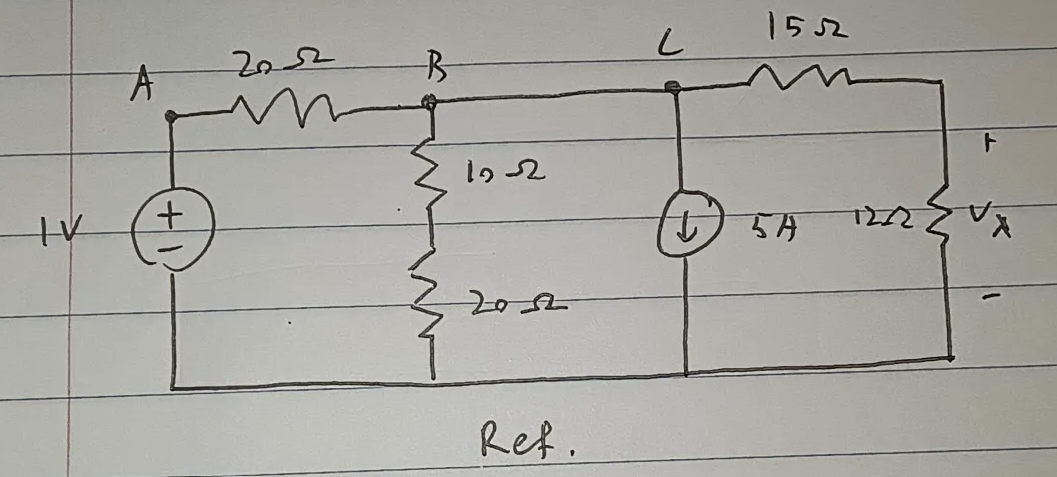
\includegraphics[width=0.5\textwidth]{7-29_2.png}
\end{center}
Node A:
\[V_A = 1 \,\text{V}\]
Node B:
\[\frac{V_A - V_B}{[20\,\Omega]} = \frac{V_B}{[10+20\,\Omega]} + [5\,\text{A}]+\frac{V_B}{[15+12\,\Omega]}\]
\[\implies -4.95 = 0.12037V_B \implies V_B = -41.123\,\text{V}\]
Since $V_C = V_B$, we can find the voltage across the 12 $\Omega$ resistor using voltage division:
\[V_x = V_C \cdot \frac{[12\,\Omega]}{[12+15\,\Omega]} = [ -41.123\,\text{V}] \cdot \frac{[12\,\Omega]}{[27\,\Omega]} = \boxed{-18.276\,\text{V}}\]
\textbf{(b)} 
\begin{center}
    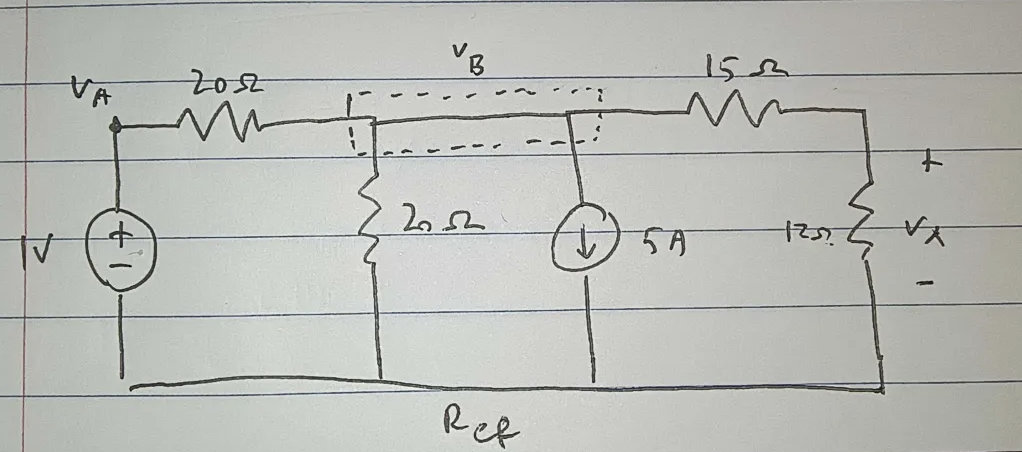
\includegraphics[width=0.5\textwidth]{7-29_3.png}
\end{center}
Node A:
\[V_A = 1 \,\text{V}\]
Node B:
\[\frac{V_A-V_B}{[20\,\Omega]} = \frac{V_B}{[20\,\Omega]}+[5\,\text{A}]+\frac{V_B}{[15+12\,\Omega]}\]
\[\implies -4.95 =0.13703V_B \implies V_B = -36.121\,\text{V}\]
We can use voltage division to find the voltage across the 12 $\Omega$ resistor:
\[V_x = V_B \cdot \frac{[12\,\Omega]}{[12+15\,\Omega]} = [ -36.121\,\text{V}] \cdot \frac{[12\,\Omega]}{[27\,\Omega]} = \boxed{-16.053\,\text{V}}\]
\textbf{(c)} 
\begin{center}
    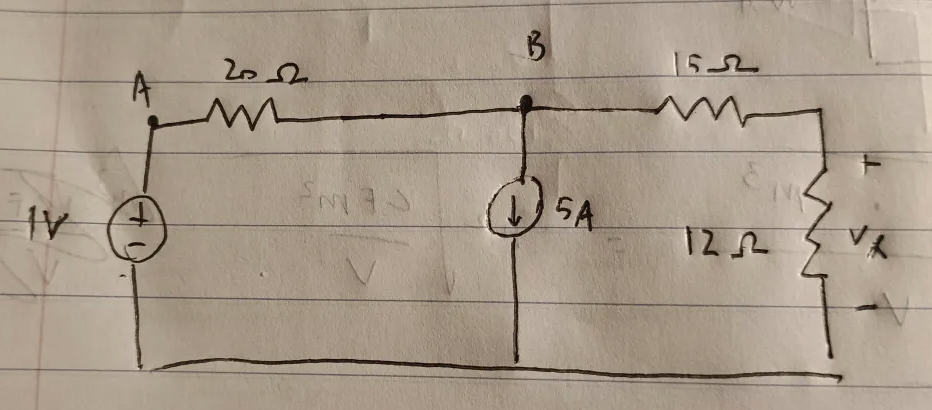
\includegraphics[width=0.5\textwidth]{7-29_4.png}
\end{center}
Node A:
\[V_A = 1 \,\text{V}\]
Node B:
\[\frac{V_A-V_B}{[20\,\Omega]} = [5\,\text{A}]+\frac{V_B}{[15+12\,\Omega]}\]
\[\implies -4.95 = 0.08703V_B \implies V_B = -56.872\,\text{V}\]
We can use voltage division to find the voltage across the 12 $\Omega$ resistor:
\[V_x = V_B \cdot \frac{[12\,\Omega]}{[12+15\,\Omega]} = [ -56.872\,\text{V}] \cdot \frac{[12\,\Omega]}{[27\,\Omega]} = \boxed{-25.276\,\text{V}}\]
\textbf{(d)} Since current flows through path of least resistance, it'll be the same case as part (b).

\section*{7.35}
\vspace{-2em}
\begin{center}
    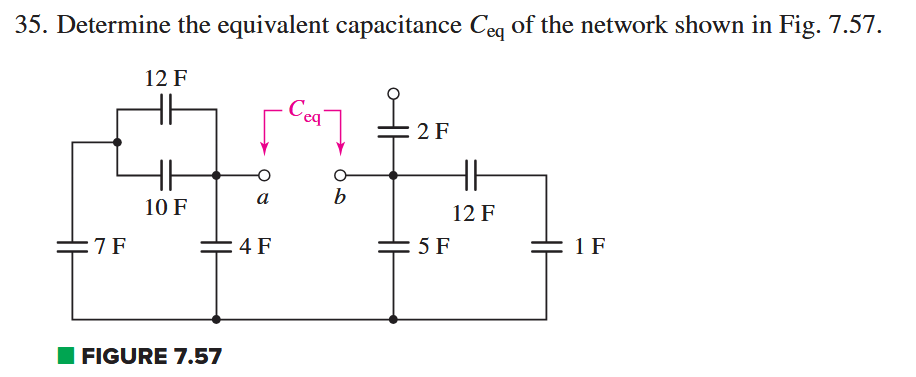
\includegraphics[width=0.8\textwidth]{7-35.png}
\end{center}
\vspace{-1em}
Capacitors in parallel add like:
\[C_{eq} = C_1 + C_2 + C_3\]
Capacitors in series add like:
\[\frac{1}{C_{eq}} = \frac{1}{C_1} + \frac{1}{C_2} + \frac{1}{C_3}\]
Working from the right: Add the 12 F and 1 F capacitors in series:
\[C_1 = \frac{[12\,\text{F}][1\,\text{F}]}{[12+1\,\text{F}]} = 0.923\,\text{F}\]
Add the 0.923 F capacitor in parallel with the 5 F capacitor:
\[C_2 = C_1 + 5 = 0.923 + 5 = 5.923\,\text{F}\]
For the left side: add the 12 F and 10 F capacitors in parallel:
\[C_3 = 12 + 10 = 22\,\text{F}\]
Add $C_3$ and 7 F in series:
\[C_4 = \frac{[22\,\text{F}][7\,\text{F}]}{[22+7\,\text{F}]} = 5.310\,\text{F}\]
Add $C_4$ and 4 F in parallel:
\[C_5 = C_4 + 4 = 5.310 + 4 = 9.310\,\text{F}\]
Finally, we have simplified both sides into 2 capacitors in series: $C_5$ and $C_2$:
\[C_{eq} = \frac{[9.310\,\text{F}][5.923\,\text{F}]}{[9.310+5.923\,\text{F}]} = \boxed{3.619\,\text{F}}\]

\section*{7.49}
\vspace{-2em}
\begin{center}
    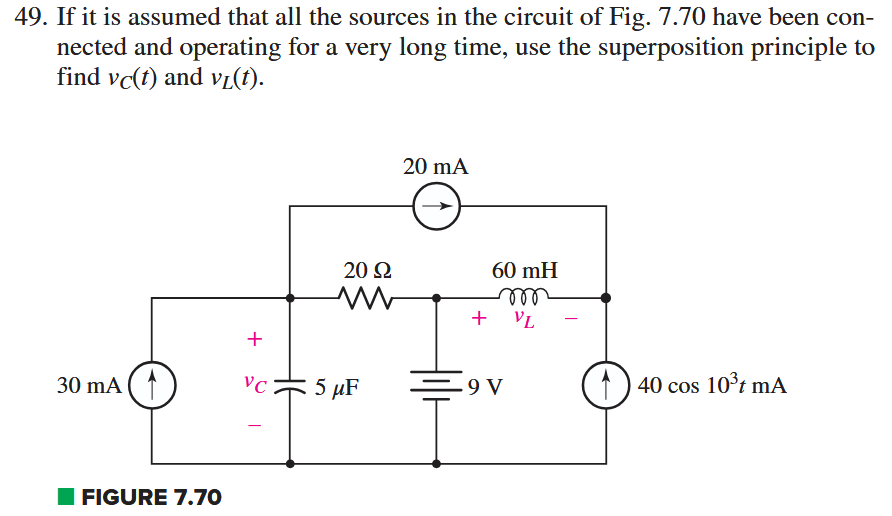
\includegraphics[width=0.8\textwidth]{7-49.png}
\end{center}
\vspace{-1em}
Using superposition, we can find the voltages across the inductor and capacitor at steady state from the DC sources and AC current source separately, and then add them together to find the total voltage across the inductor and capacitor.\\\\
\textbf{DC sources only}: Following superposition, turning off the current source becomes an open circuit. Redrawing the circuit at steady state:
\begin{center}
    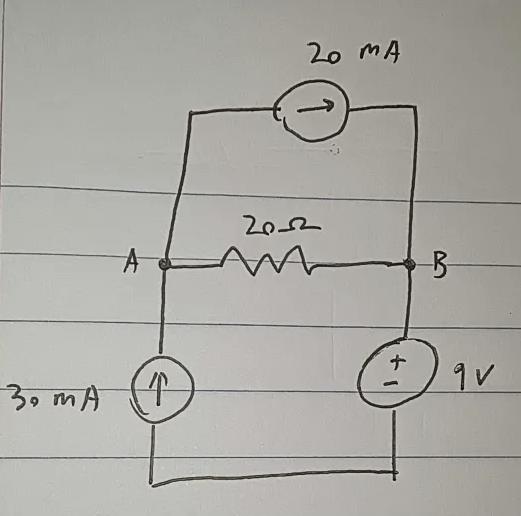
\includegraphics[width=0.4\textwidth]{7-49_1.png}
\end{center}
At steady state, $\frac{di}{dt}=0$ so the inductor has a voltage of 
\[\underline{V_{L,DC} = 0\,\text{V}}\]
The capacitor has a voltage equal to $V_A$. We can find $V_A$ using nodal analysis:\\\\
Node A:
\[[30\times10^{-3}\,\text{A}] = \frac{V_A - V_B}{[20\,\Omega]} +[20\times10^{-3}\,\text{A}]\]
Node B:
\[V_B = 9\,\text{V}\]
\[\implies V_A  = 9.2\,\text{V}\implies \underline{V_{C,DC} = 9.2\,\text{V}}\]
\textbf{AC current source only}: Following superposition, turning off the voltage sources becomes short circuits, and current sources becomes open circuits. Redrawing the circuit at steady state:
\begin{center}
    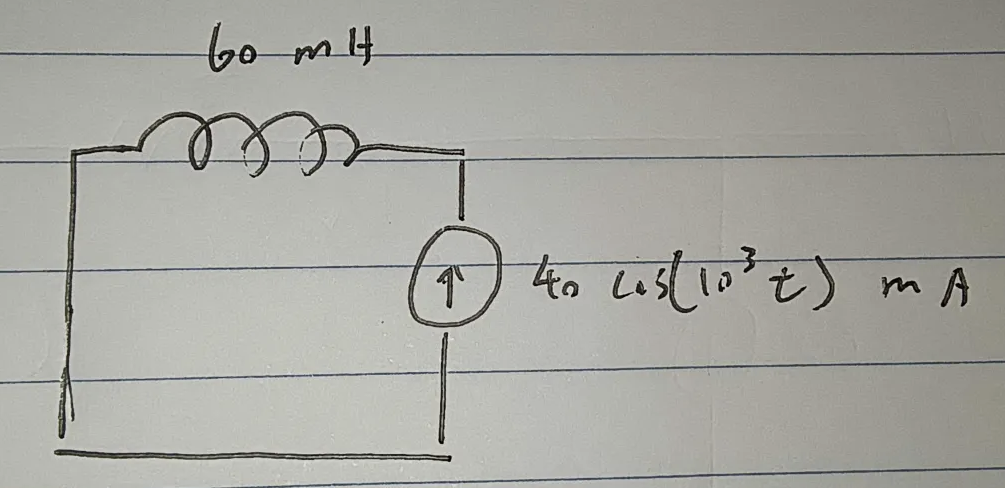
\includegraphics[width=0.5\textwidth]{7-49_2.png}
\end{center}
Since the voltage source becomes a short circuit, the capacitor then has a voltage of zero (no current flows through it):
\[\underline{V_{C,AC} = 0\,\text{V}}\]
For the inductor, we can differentiate the current to find the voltage across it:
\[V_{L,AC} = L\frac{di}{dt} = [60\times10^{-3}\,\text{H}]\cdot\frac{d}{dt}[40\cos(1000t)\times10^{-3}\,\text{A}] = \underline{-2.4\sin(1000t)\,\text{V}}\]
Finally, applying superposition:
\[\boxed{V_C = V_{C,DC} + V_{C,AC} = 9.2\,\text{V} + 0\,\text{V} = 9.2\,\text{V}}\]
\[\boxed{V_L = V_{L,DC} + V_{L,AC} = 0\,\text{V} - 2.4\sin(1000t)\,\text{V} = -2.4\sin(1000t)\,\text{V}}\]

\section*{7.54}
\vspace{-2em}
\begin{center}
    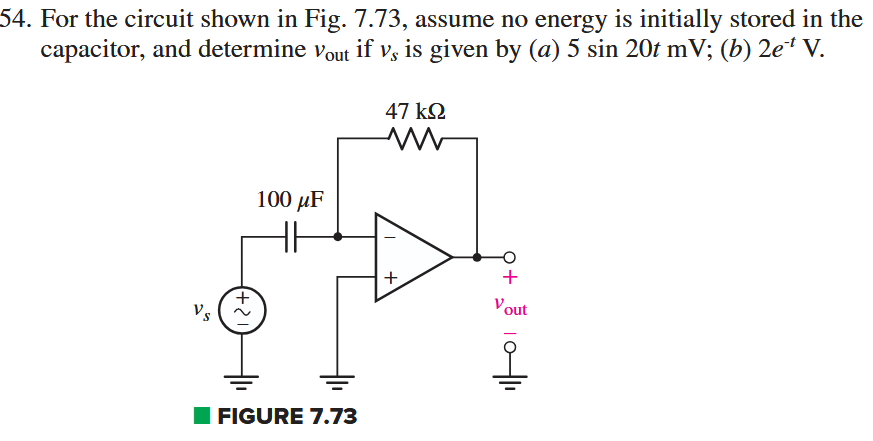
\includegraphics[width=0.8\textwidth]{7-54.png}
\end{center}
\vspace{-1em}
Since the non-inverting terminal of the op amp is grounded, the inverting terminal will also be at 0 V. Thus, the voltage drop across the capacitor must be equal to the voltage source $V_s$.
\[V_C = V_s - [0\,\text{V}]\]
Applying KCL at the node between the capacitor and the 47 k$\Omega$ resistor:
\[i_C = i_R\]
Where $i_C$ is found through differentiating the voltage across the capacitor:
\[V_C = \frac{Q}{C} \implies \frac{dV_C}{dt} = \frac{1}{C}\frac{dQ}{dt}\]
\[\implies i_C = C\frac{dV_s}{dt}\]
$i_R$ is found through Ohm's law:
\[i_R = \frac{0-V_\text{out}}{[47\times10^3\,\Omega]}\]
Setting them equal to each other:
\[C\frac{dV_s}{dt} = \frac{0-V_\text{out}}{[47\times10^3\,\Omega]} \implies V_\text{out} = -[47\times10^3\,\Omega][100\times10^{-6}\,\text{F}]\frac{dV_s}{dt}\]
Simplified:
\[V_\text{out} = -4.7\frac{dV_s}{dt}\,\text{[V]}\]
\textbf{(a)} $V_s = 5\sin(20t)$ mV
\[\frac{dV_s}{dt} = 5 \cdot 20 \cos(20t)\,\text{mV/s}  = 100 \cos(20t)\times 10^{-3}\,\text{V/s}\]
\[V_\text{out} = -4.7(0.1\cos(20t)) = \boxed{-0.47\cos(20t)\,\text{V}}\]
\textbf{(b)} $V_s = 2e^{-t}$ V
\[\frac{dV_s}{dt} = -2e^{-t}\,\text{V/s}\]
\[V_\text{out} = -4.7(-2e^{-t}) = \boxed{9.4e^{-t}\,\text{V}}\]

\end{document}